93. \begin{figure}[ht!]
\center{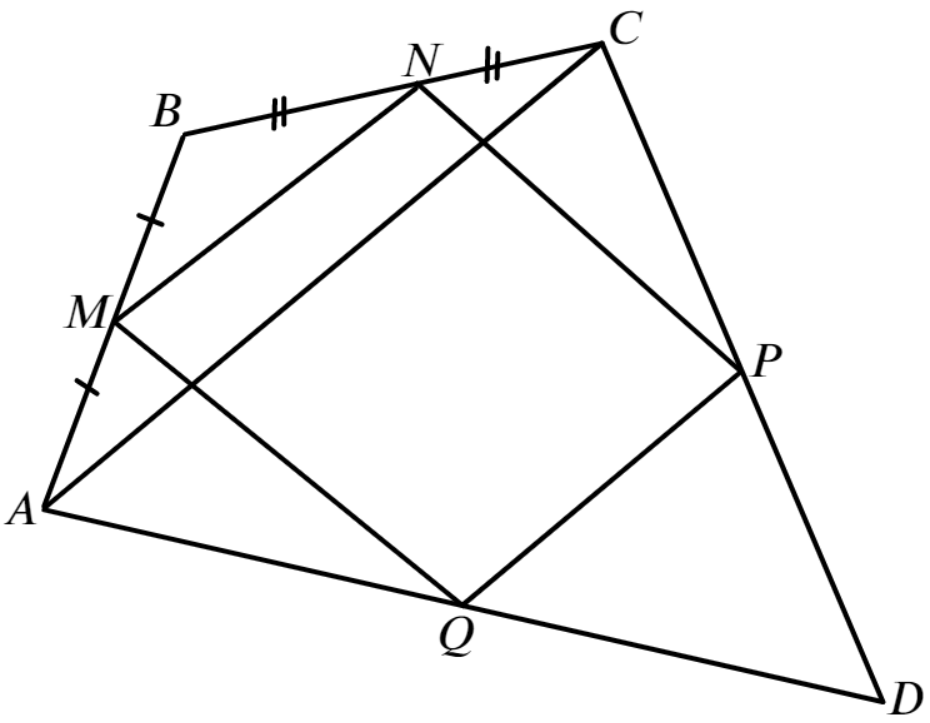
\includegraphics[scale=0.35]{g8-92.png}}
\end{figure}\\
Проведём диагональ $AC,$ тогда $MN$ является средней линией в треугольнике $ABC$ и треугольник $ABC$ подобен треугольнику $MBN$ с коэффициентом 2 (по двум сторонам и общему углу между ними), значит $S_{\Delta MBN}=\cfrac{1}{4}S_{\Delta ABC}.$ Аналогично $S_{\Delta DPQ}=\cfrac{1}{4}S_{\Delta ACD},\  S_{\Delta CNP}=\cfrac{1}{4}S_{\Delta BCD},\ S_{\Delta AMQ}=\cfrac{1}{4}S_{\Delta ABD}.$ Пусть $S_{ABCD}=S_1,$ тогда $S_{MNPQ}=S_1-S_{\Delta MBN}-S_{\Delta DPQ}-S_{\Delta CNP}-S_{\Delta AMQ}=
S_1-\cfrac{1}{4}S_{\Delta ABC}-\cfrac{1}{4}S_{\Delta ACD}-\cfrac{1}{4}S_{\Delta BCD}-\cfrac{1}{4}S_{\Delta ABD}=S_1-\cfrac{1}{4}(S_{\Delta ABC}+S_{\Delta ACD}+
S_{\Delta BCD}+S_{\Delta ABD})=S_1-\cfrac{1}{4}\cdot2S_1=\cfrac{S_1}{2},$ значит $S_1=2S.$\\
